% !TeX root = ../presentation.tex



\section{Constrained Attitude Control}
\subsection{Motivation}

\begin{frame}[t]{Motivation} %-----------------------------%
\begin{itemize}
    \item Autonomous control of space vehicles is critical
    \begin{itemize}
        \item Avoid extensive planning and interaction by operators
        \item Ability to operate safely with system uncertainty 
        \item Independently navigate hazards and handle possible failures
    \end{itemize}
\end{itemize}
\visible<2->{
\begin{figure} 
    \centering  
    \begin{subfigure}[b]{0.5\textwidth} 
        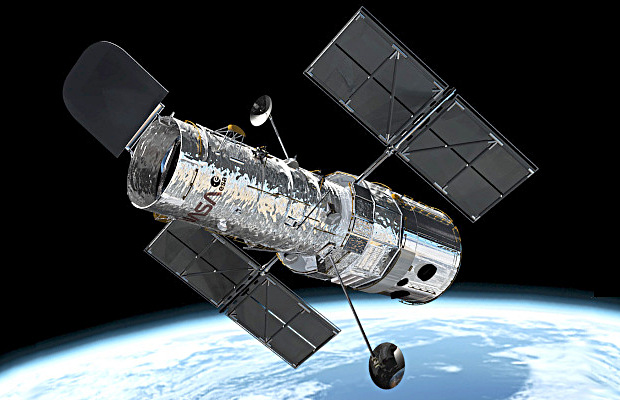
\includegraphics[height=0.5\textheight]{figures/2016ACC/hubble.jpg}
    \end{subfigure}~
    \begin{subfigure}[b]{0.5\textwidth} 
        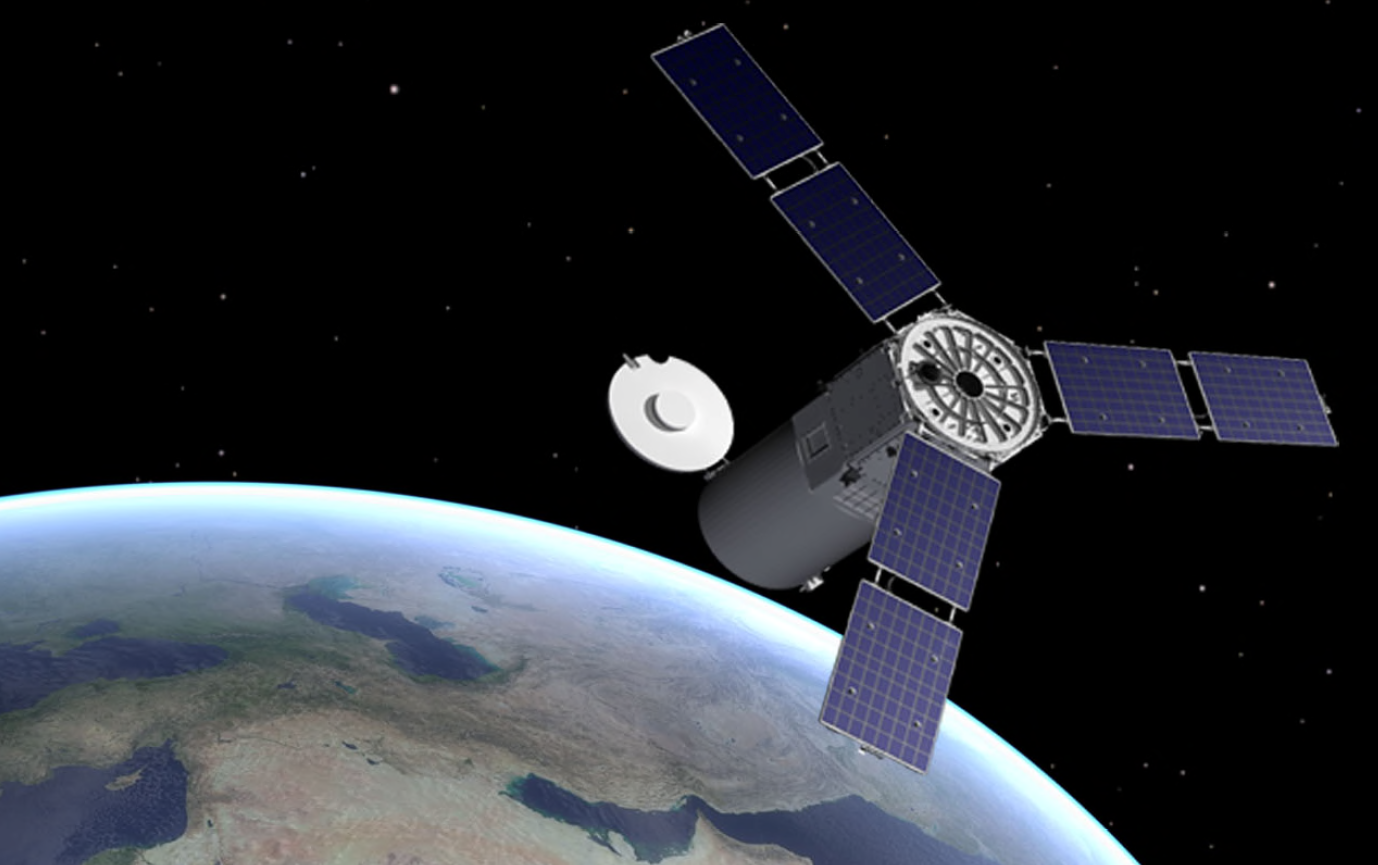
\includegraphics[height=0.5\textheight]{figures/2016ACC/ors-1.png}
    \end{subfigure}
\end{figure}
}
\end{frame}   %-----------------------------%


\begin{frame}[t]{Problem Formulation} %-----------------------------------%
\begin{itemize}
    \item \Emph{Constrained attitude control} : reorient vehicle while avoiding pointing at obstacles
    \begin{itemize}
        \item Exclusion zones for payloads e.g infrared telescope
        \item UAVs manuevering in congested locations
        \item Laser/Radio emitters on spacecraft
    \end{itemize}
    \pause
    \vs
    \item Previous approaches have several issues
    \begin{itemize}
        \item Attitude parameterizations: singularities/ambiguities
        \item Ad-hoc path planning: difficult to generalize to arbitrary obstacles
        \item Randomized methods: lack of stability guarantees
        \item Optimization based: expensive to compute and only provides open-loop control  
    \end{itemize}
\end{itemize}
\end{frame} %-------------------------------------%

\begin{frame}{Attitude Parameterizations}
    \begin{itemize}
        \item Euler Angles
        \begin{itemize}
            \item Minimal representation used for small attitude changes.
            \item Singularities exist for large angle slews: requires switching between 24 sequences
            \item Complicated trigonometric functions
        \end{itemize}
        \pause
        \vs
        \item Quaternion 
        \begin{itemize}
            \item No singularities
            \item Two anti-podal quaternions for the same attitude
            \item Unwinding behavior for control systems
        \end{itemize}
        \pause
        \vs
        \item Geometric control
        \begin{itemize}
            \item Globally and uniquely characterize attitude: \( R \in \SO \)
            \item Controller is globally valid for large angle maneuvers
        \end{itemize}
    \end{itemize}
    
\end{frame}

\subsection{Approach}

\begin{frame}{Objective} %---------------------------------------%

    \begin{block}{Nonlinear Control Design}
        Design control input \( u \) that stabilizes system from initial attitude \( R_0 \) to desired attitude \( R_d \) while avoiding obstacles
    \end{block}
    \pause
    \vs
    \begin{itemize}
        \item Avoid drawbacks of other approaches 
        \begin{itemize}
            \item \Emph{Geometric control} - analysis is conducted directly on \( \SO \) 
            \item \Emph{Barrier function} - allows for arbitrary amount of constraints
            \item \Emph{Efficient } - real time feedback control
            \item \Emph{Stability} - Lyapunov analysis gives rigourous stability proof
            \item \Emph{Adaptive} - handles system uncertainties
        \end{itemize}
    \end{itemize}
\end{frame}


\begin{frame}{Spacecraft Orientation} %-----------------------------%

\begin{itemize}

    \item \Emph{Attitude Representation}: rotation matrix from body to inertial frame
     \[\SO =  \{R\in\R^{3\times 3}\,|\, R^TR=I,\;\mathrm{det}[R]=1\} . \]
    \item Rigid body attitude dynamics:
    \begin{gather*}
        J\dot\Omega + \Omega\times J\Omega = u+W(R,\Omega)\Delta , \quad \dot R = R\hat\Omega .
    \end{gather*}

    \item Sensor and obstacles defined by unit vectors in \( \R^3 \) 
        \begin{itemize}
            \item Body fixed sensor: \( r \in \S^2\)
            \item Inertially fixed hazard: \( v \in \S^2 \)
        \end{itemize} 
    \vs
    \item Hard cone constraint: \( r^T R^T v \leq \cos \theta \)
    
\end{itemize}
\end{frame}   %-----------------------------%

  
\subsection*{Error Function}

\begin{frame}{Configuration Error Function} %-----------------------------%
\only<1>{
\begin{itemize}
    \item Error function quantifies ``distance'' to desired attitude
    \begin{align*}
            \Psi(R, R_d) = A(R, R_d) B(R) .
    \end{align*}
    \vs
    \item Combination of attractive and repulsive terms   
\end{itemize}
\begin{gather*}
    A(R, R_d) = \frac{1}{2} \tr{G \left( I - R_d^T R\right)} . \\ \\
    B_i(R) = 1 - \frac{1}{\alpha_i} \ln \left( - \frac{ r^T R^T v_i - \cos \theta_i}{1 + \cos \theta_i}\right) .
\end{gather*}     
}

\only<2>{
    \begin{itemize}
        \item Attractive well at the desired attitude
    \end{itemize}
    \begin{align*}
        A(R,R_d) = \frac{1}{2} \tr{G \left( I - R_d^T R\right)} .
    \end{align*}
    \begin{figure} 
        \centering
        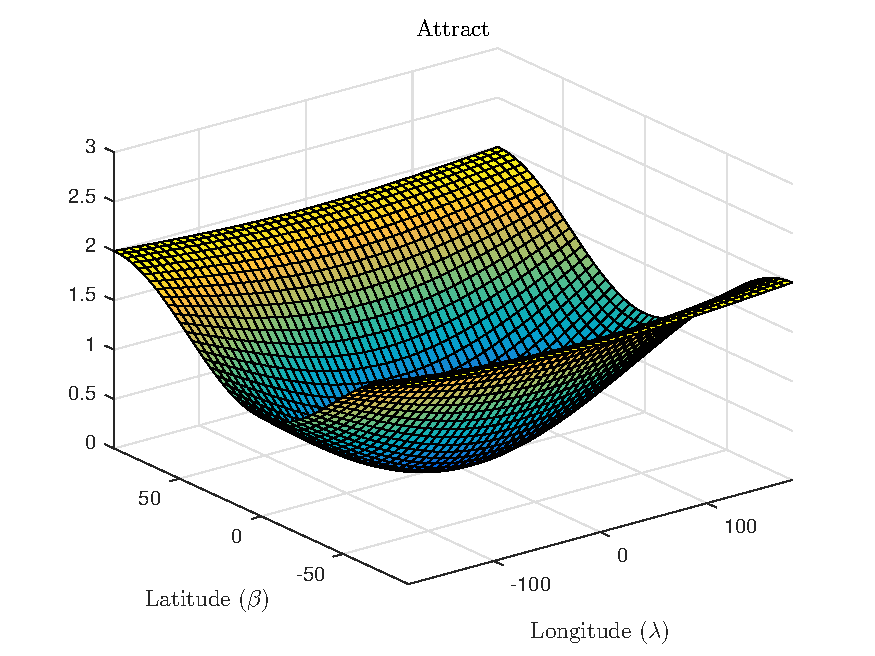
\includegraphics[height=0.6\textheight]{figures/2016ACC/attract_error.pdf}
    \end{figure}
}

\only<3>{
    \begin{itemize}
        \item Define a barrier around obstacles
    \end{itemize}
    \begin{align*}
        B_i(R) = 1 - \frac{1}{\alpha_i} \ln \left( - \frac{ r^T R^T v_i - \cos \theta_i}{1 + \cos \theta_i}\right).
    \end{align*}
    \begin{figure}
        \centering
        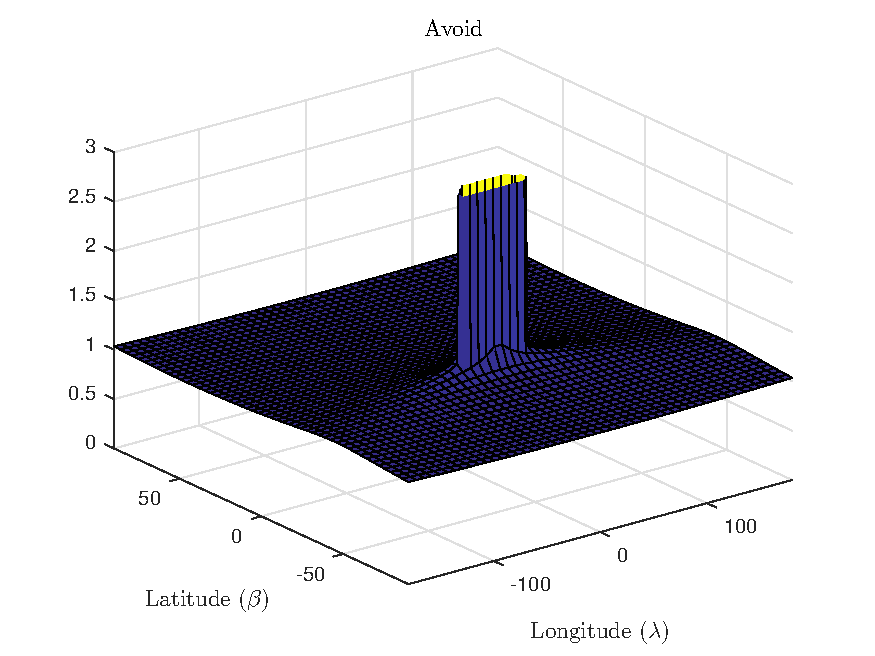
\includegraphics[height=0.6\textheight]{figures/2016ACC/avoid_error.pdf}
    \end{figure}

}

\only<4>{
    \begin{itemize}
        \item Configuration error: \( \Psi : \Q \times \Q \to \R \) with control chosen to follow slope of \( \Psi \) to minimum at \( R_d\)
    \end{itemize}
    \begin{align*}
        \Psi(R, R_d) = A(R,R_d) B(R) .
    \end{align*}
    \begin{figure}
        \centering
        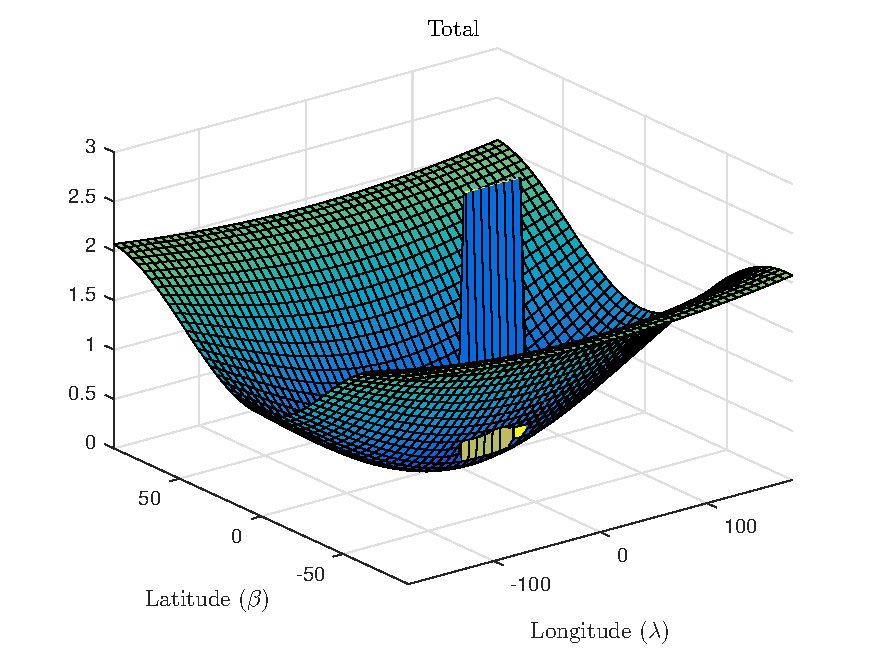
\includegraphics[height=0.6\textheight]{figures/2016ACC/combined_error.pdf}
    \end{figure}
}
\end{frame}   %-----------------------------%

\begin{frame}{Attitude Error Vectors} % -----------------------------------------------%
    \begin{itemize}
        \item Define attitude and velocity error vectors in tangent space 
        \item Variation of \( \Psi \) expressed in terms of Lie algebra - \( \delta R = R \hat{\eta} \) for \( \eta \in \R^3 \)
        \begin{align*}
            \dirDiff{A}{R} &= \eta \cdot e_{R_A} ,\\
            \dirDiff{B}{R} &= \eta \cdot e_{R_{B}} . 
        \end{align*}
        \item With these error variables, we can formulate a PD-like control on \( \SO \)
        \begin{gather*}
            \Psi(R, R_d) = A(R, R_d) B(R) , \label{eqn:psi} \\
            e_R = e_{R_A} B(R) + A(R,R_d) e_{R_B} , \label{eqn:eR} \\
            e_\Omega = \Omega .   \label{eqn:eW} 
        \end{gather*}
        
    
    \end{itemize}
    
\end{frame} %--------------------------------------------------%

\subsection*{Controller}

\begin{frame}{Adaptive Attitude Control} %-----------------------------%
\begin{itemize}
    \item Incorporate an adaptive control term to handle unknown disturbances, e.g.\ Stuck actuator or gravity gradient moment
\end{itemize}
\pause
\vs
    \begin{block}{Adaptive Attitude Controller}
        Zero equilibrium of error vectors are Lyapunov stable, furthermore \( e_R , e_\Omega \to 0 \) as \( t \to \infty \)
        \begin{align*}
            u &= - k_R e_R - k_{\Omega} e_{\Omega} + \Omega \times J \Omega - W \bar{\Delta}, \\
            \dot{\bar{\Delta}} &= k_\Delta W^T \parenth{ e_\Omega + c e_R } .
        \end{align*}
    \end{block}
    
\end{frame}   %-----------------------------%

\begin{frame}[label=proof]{Lyapunov Analysis}
\begin{itemize}
    \item Positive definite Lyapunov function
    \begin{align*}
        \mathcal{V} = \frac{1}{2} e_\Omega \cdot J e_\Omega + k_R \Psi + c J e_\Omega \cdot e_R + \frac{1}{2 k_\Delta} e_\Delta \cdot e_\Delta . \label{eqn:v_adapt}
    \end{align*}
    \pause
    \item Define upper bound of \( e_R, \dot{e}_{R}\)
    \item Upper bound of \( \dot{\mathcal{V}} \) with \(\zeta=[\|e_R\|,\|e_\Omega\|]\in\R^2\)
    \begin{align*}
        \dot{\mathcal{V}} \leq -\zeta^T M \zeta .
    \end{align*}
    \pause
    \item LaSalle-Yoshizawa theorem implies that \(\lim_{t\to\infty} \zeta=0\) 
    \item Estimation error \( e_\Delta \) is bounded since \( \mathcal{V} \) is non-increasing
\end{itemize}
\end{frame}


\subsection*{Simulation}

\begin{frame}{Numerical Simulation} %-----------------------------%

\begin{itemize}
    \item Simulate a S/C completing a yaw rotation
    \item Single obstacle in the path of sensor
\end{itemize}

\begin{center}
    \animategraphics[autoplay,loop,width=0.75\textheight]{8}{./animation/2016ACC/single_noavoid/single_noavoid-}{0}{99}~
    \animategraphics[autoplay,loop,width=0.75\textheight]{8}{./animation/2016ACC/single_avoid/single_avoid-}{0}{99}
\end{center}

\end{frame}%-----------------------------%

\begin{frame}{Multiple obstacles}%-------------------------------------%

\begin{itemize}
    \item Easily handle multiple arbitrary constraints 
    \begin{align*}
        \Psi = A(R) \bracket{1 + \sum_i C_i(R)} \quad C_i = B(R) - 1
    \end{align*}
\end{itemize}

\begin{figure}
    \centering
    \animategraphics[autoplay,loop,width=0.65\textheight]{8}{./animation/2016ACC/multiple_avoid/multiple_avoid-}{0}{99}
\end{figure}

\end{frame}%---------------------------------------%

\subsection*{Experiment}

\begin{frame}{Hexrotor Design} %--------------------%
    \begin{itemize}
        \item Three pairs of counter-rotating propellers, angled at \SI{15}{\degree}
        \item Multi-threaded C on Linux ODROID XU3
        \item Onboard IMU measures angular velocity and Vicon motion capture system for attitude
        \item Controlled remotely via SSH connection
    \end{itemize}
    
    \begin{figure} 
        \centering 
        \begin{subfigure}[b]{0.4\textwidth} 
            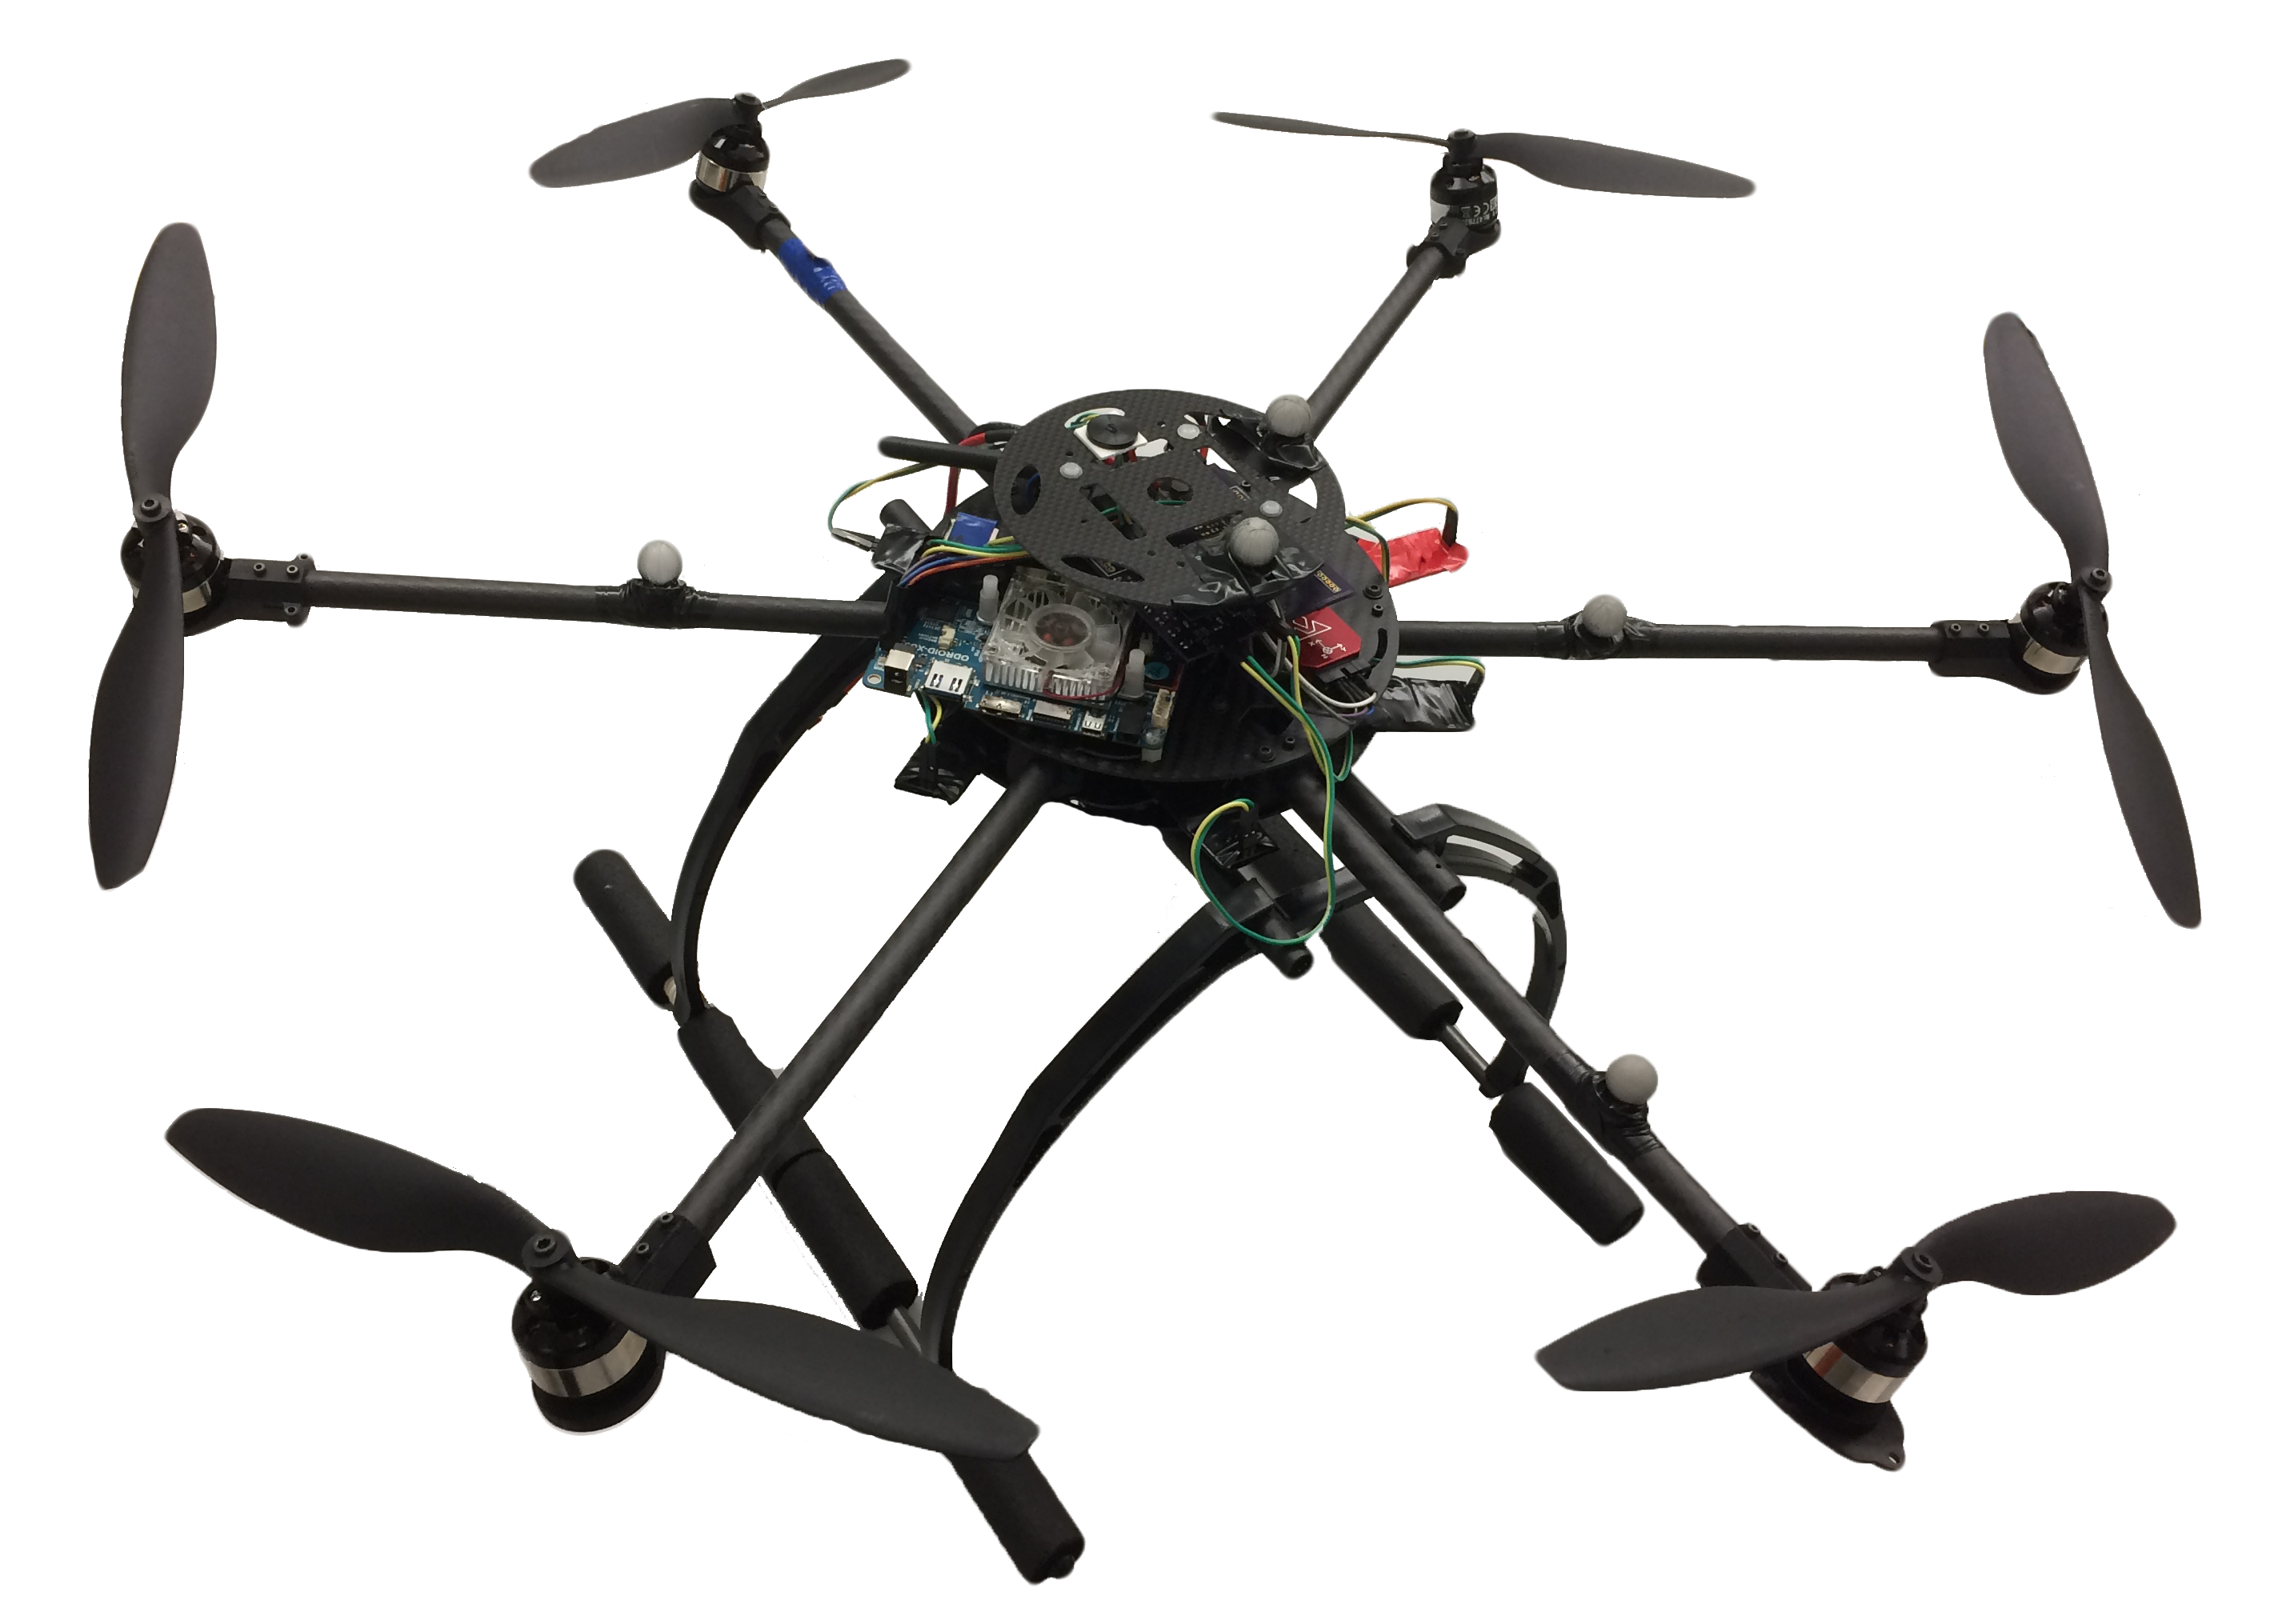
\includegraphics[height=0.4\textheight]{figures/2016ACC/hexrotor_no_background.png} 
        \end{subfigure}~ %add desired spacing between images, e. g. ~, \quad, \qquad, \hfill etc. %(or a blank line to force the subfigure onto a new line) 
        \begin{subfigure}[b]{0.4\textwidth} 
            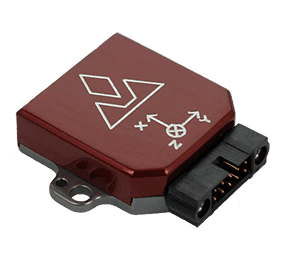
\includegraphics[height=0.4\textheight]{figures/2016ACC/vn-100-rugged.png}
        \end{subfigure}
    \end{figure}
\end{frame} %-----------------------%

\begin{frame}{Hexrotor Experiment} %-----------------------------%
\begin{itemize}
    \item Attached to spherical joint to allow only attitude dynamics
\end{itemize}
\begin{figure}
\centering
\movie[externalviewer,height=0.7\textheight]{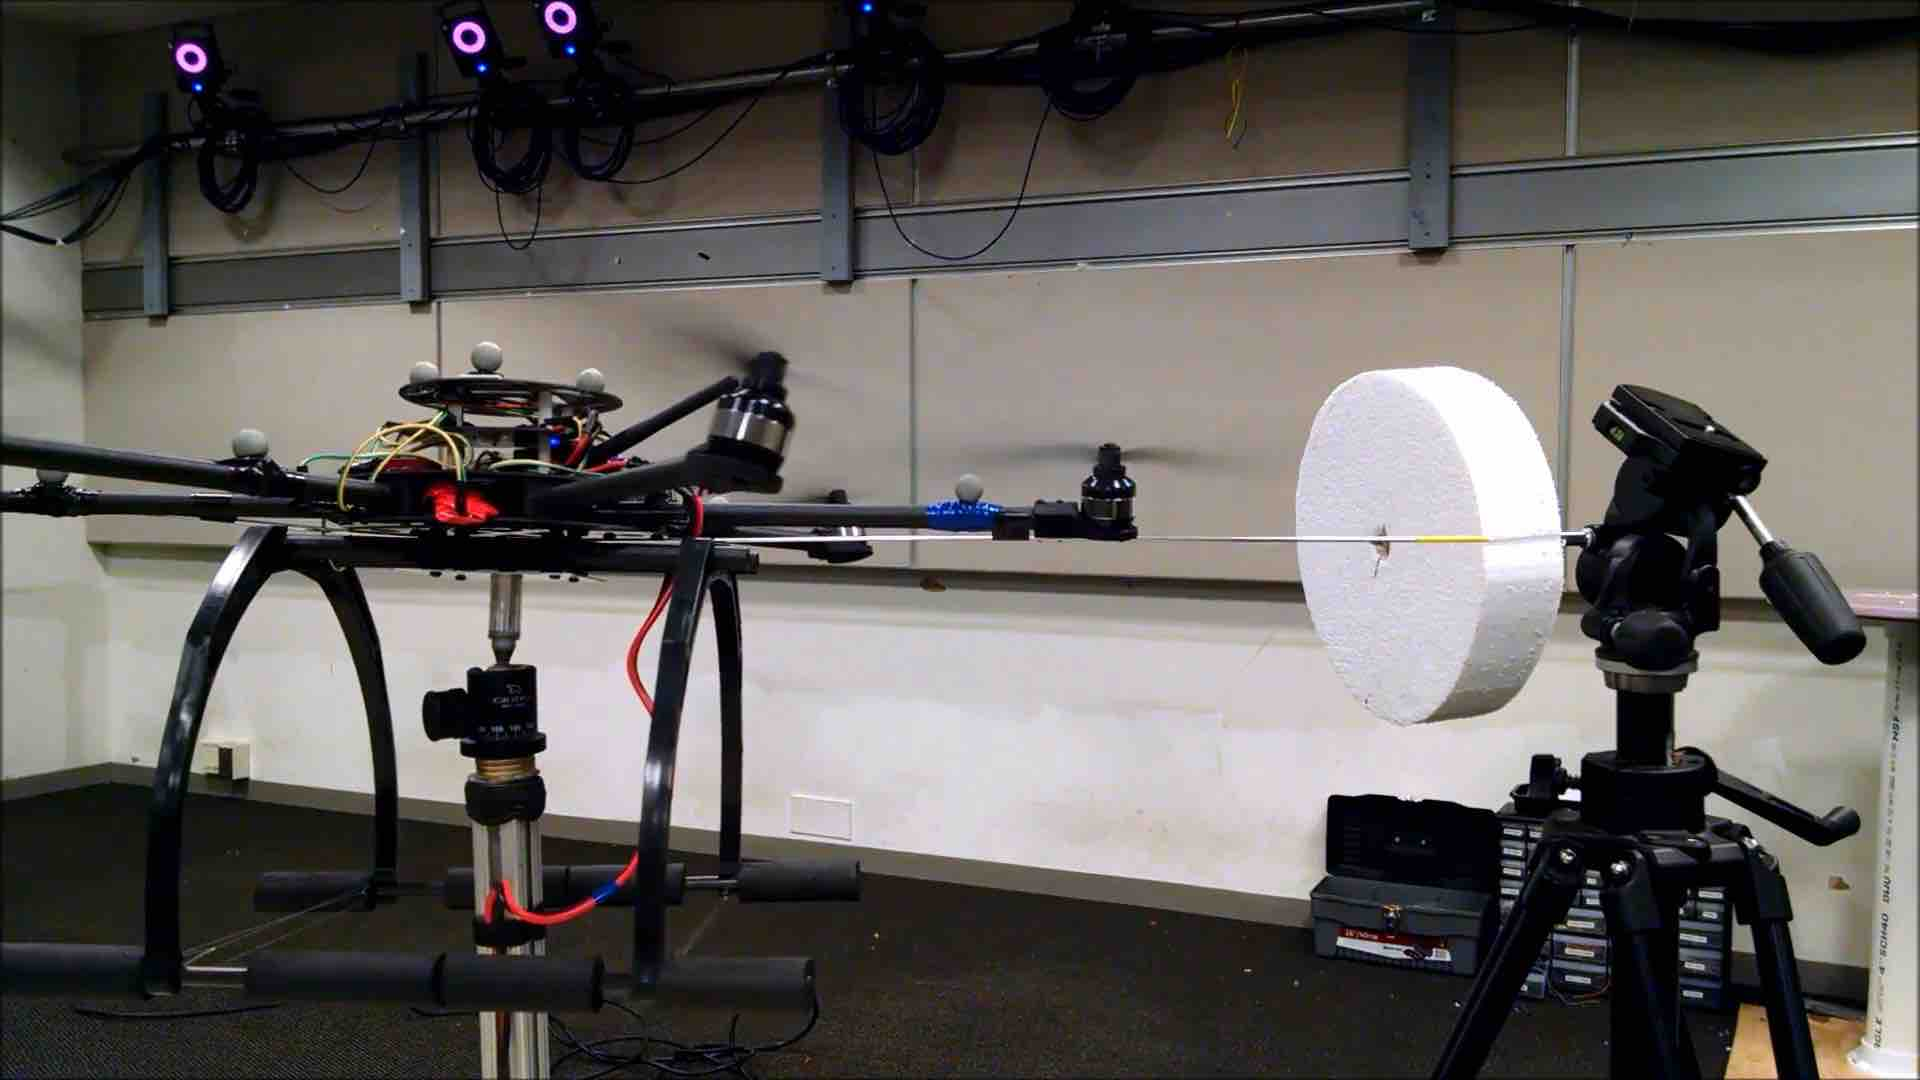
\includegraphics[height=0.7\textheight]{figures/2016ACC/hexrotor.jpg}}{videos/experiment.mp4} 
\end{figure}
\end{frame}   %-----------------------------%

